\section{Caching}

\begin{frame}{Intro}

	Solution: Caching\\
	\spc
	Caching is:
	\begin{itemize}
		\item We have a slow medium
		\item Add a fast medium in a data path
		\item Transparently store the data that are intended for the 
			slower medium.
		\item Profit: later accesses to the same data are faster
	\end{itemize}
	\dspc
	Sounds familiar?

	\note[item]{Η κλασσική λύση σε τέτοια προβλήματα είναι η χρήση ενός 
		γρηγορότερου αποθηκευτικού μέσου για caching.}
	\note[item]{Για όσους δεν ξέρουν τι σημαίνει caching, θα το εξηγήσουμε 
		συνοπτικά: έχεις ροή, αργό μέσο, βάζεις ένα γρήγορο, speedup}
	\note[item]{Προφανώς αυτό το concept είναι γνωστό. Από που;}
\end{frame}

\begin{frame}
	\makebox[\textwidth]{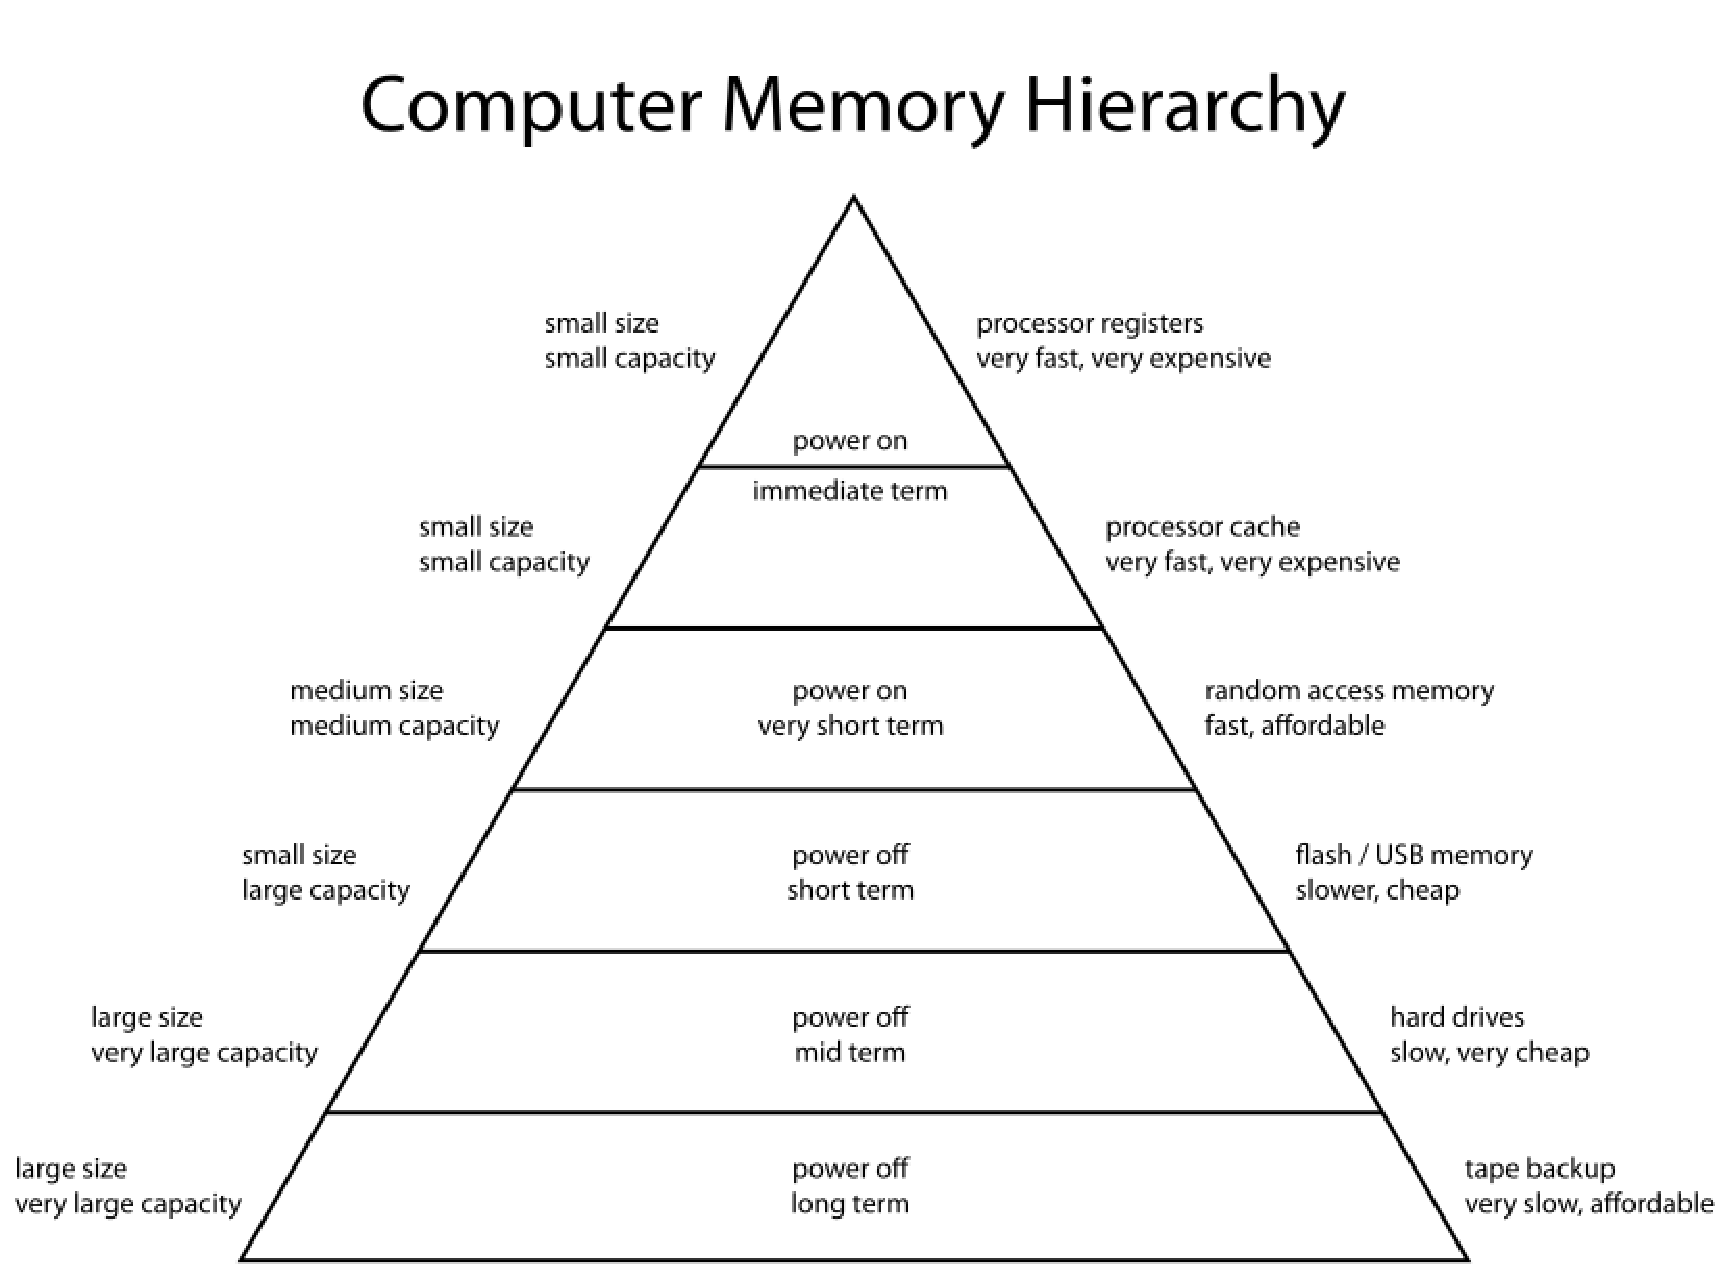
\includegraphics[width=0.8\textwidth]{images/mem-hier.pdf}}
	
	That's because every PC is built that way.

	\note[item]{Από το ιεραρχικό μοντέλο του υπολογιστή: cpu cache vs ram, ram 
		vs disk}
\end{frame}

\begin{frame}
	Is there anything to help us?
	\dspc
	FACT: We are not the first to have speed issues\\
	Facebook, Twitter, Dropbox, every one has hit and surpassed their limits.
	\dspc
	There are solutions separated in two categories:
	\begin{itemize}
		\item Block store
		\item Key-value store
	\end{itemize}
	\note[item]{Τώρα που ξέρουμε τη λύση, υπάρχει κάτι που μπορούμε να 
		κάνουμε;}
	\note[item]{Υπάρχει κάτι έτοιμο; ΝΑΙ}
	\note[item]{Δυο κατηγορίες:
		\begin{itemize}
			\item βλέπουν τα δεδομένα σαν blocks ενός δίσκου
			\item βλέπουν τα δεδομένα σαν κομμάτια αντικειμένων
		\end{itemize}
		Διαφορά: \todo
	}
\end{frame}

\begin{frame}{Block-store caching solutions}

	Most notable examples:
	\begin{itemize}
		\item Bcache
		\item Flashcache
		\item EnhanceIO
	\end{itemize}
	\dspc
	Typically scale-up solutions.
	\dspc
	Pros: Simple, scale-up\\
	Cons: Unaware of CoW, kernel solutions

	\note[item]{Πρώτη κατηγορία που εξετάσαμε έχει αρκετά ενδιαφέρουσες 
		λύσεις.}
	\note[item]{Δε θα επεκταθούμε γιατί έχουν κάποια βασικά κοινά:
		\begin{itemize}
			\item Kernel modules
			\item expose εικονικά block devices
		\end{itemize}
	}
	\note[item]{Εξήγησε που μπαίνουν (xsegbd)}

\end{frame}

\begin{frame}{Key-value caching solutions}
	Most notable examples:
	\begin{itemize}
		\item Memcached
		\item Couchbase
	\end{itemize}
	\dspc
	Typically scale-out solutions
	\dspc
	Pros: Distributed with no SPOF, can utilize unneeded RAM\\
	Cons: Memcached has no persistence, Couchbase cannot use RADOS as its 
	backend, more suitable for databases
\end{frame}

\begin{frame}{Page-cache}

	What if we used the page-cache?

	\dspc
	Pros: Easy to activate, tested, very fast\\
	Cons: Unaware of CoW, no control over it, practically kernel solution\\

\end{frame}

\begin{frame}{Conclusions}

	\begin{itemize}
		\item Most solutions far from Archipelago's logic
		\item Block store might be good for the storage backend
		\item Must implement our own solution
	\end{itemize}
\end{frame}
	
